In this chapter, we present the empirical findings derived from our computational experiments.


\section{Comparison of Mean Values}
\begin{sidewaysfigure}[p]
    \centering
    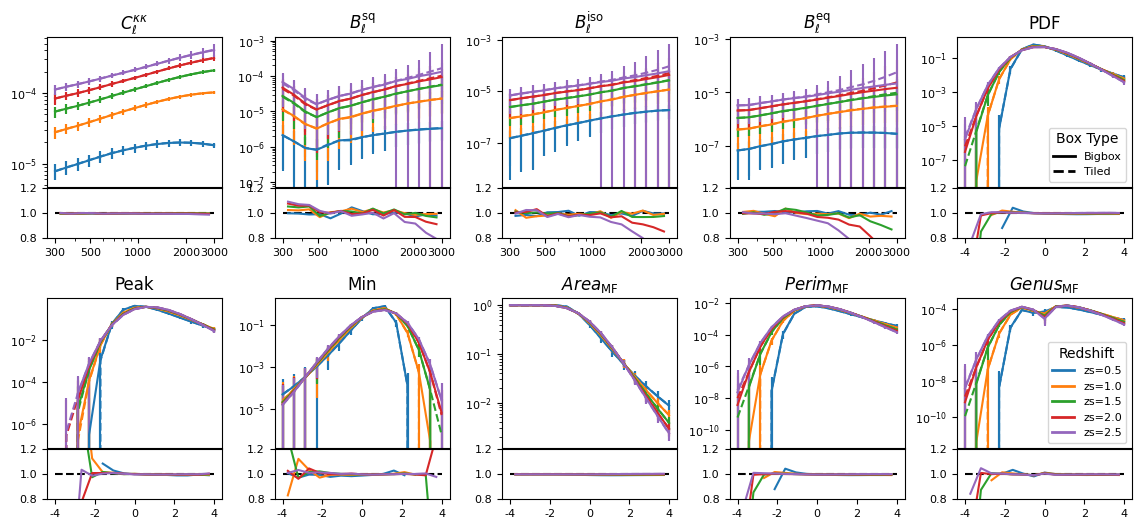
\includegraphics[width=\textwidth]{figures/mean_final.png}
    \caption{Mean values of various statistical measures across all flat patches for different source redshifts ($z_s = 0.5, 1.0, 1.5, 2.0, 2.5$), comparing the BIGBOX (solid lines) and TILED (dashed lines) simulations. The top row includes the angular power spectrum ($C^{KK}_{\ell}$), bispectrum for three configurations (square, isosceles, and equilateral), and the probability density function (PDF). The bottom row presents peak counts, minima, and Minkowski Functionals (area, perimeter, and genus). The lower subplots in each panel depict the ratio of TILED to BIGBOX values, with a baseline set at unity (1.0), indicating agreement between the simulations.}
    \label{fig:mean}
\end{sidewaysfigure}
Figure~\ref{fig:mean} shows the mean values of a comprehensive set of statistical measures across all flat patches for source redshifts ($z_s = 0.5, 1.0, 1.5, 2.0, 2.5$). This comparison contrasts results from the BIGBOX simulations (solid lines) with those from the TILED simulations (dashed lines). The lower subplots in each panel display the ratio of TILED to BIGBOX values, with a baseline of unity (1.0) to gauge concordance between the two simulation methods. Deviations from unity indicate discrepancies due to super-sample covariance (SSC) and tiling effects. Ratios clustering around the baseline confirm consistency and reliability across various statistical measures and source redshifts.

Most mean values align well between the BIGBOX and TILED simulations, with exceptions in two regimes: the low $\kappa/\sigma_\kappa$ region and the high multipole moment ($\ell$) range of the bispectra. The low $\kappa/\sigma_\kappa$ discrepancy stems from lack of particle number, resulting in more void regions in TILED simulations. The high-$\ell$ discrepancy arises from tiling effects, or the Box Replication Effect (\citealt{2024MNRAS.534.1205C}), which emphasizes overdense (underdense) region bias by its repetitive nature.

It is worth noting that the PDF, peak counts, minima, and Minkowski Functionals exhibit minimal discrepancies between the two simulation methods. This finding suggests that these higher order statistics are less sensitive to tiling effects.

\section{Impact on Covariance Matrices}
\begin{sidewaysfigure}[h]
    \centering
    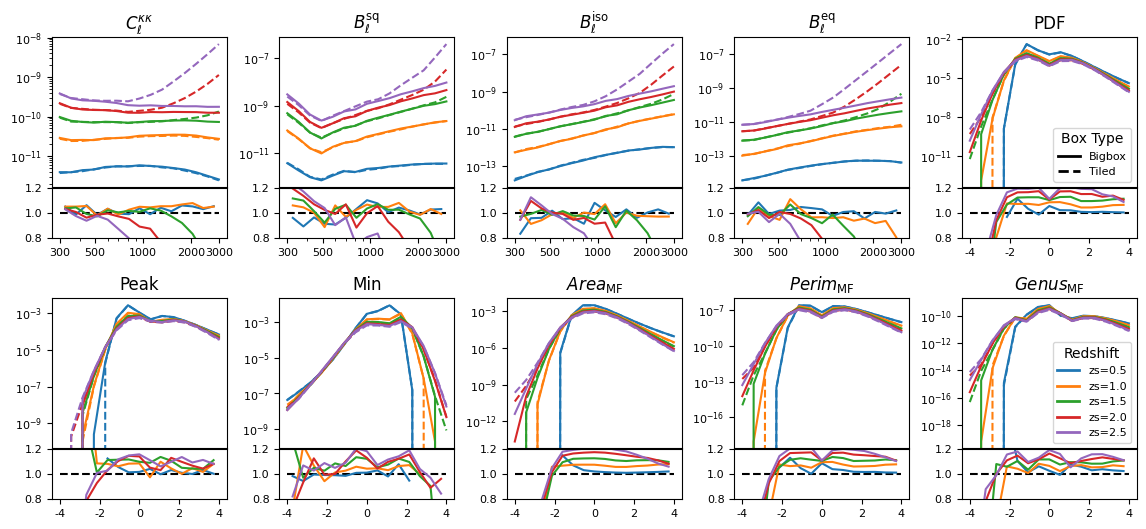
\includegraphics[width=\textwidth]{figures/diag_final.png}
    \caption{Diagonal elements of the covariance matrices for the same set of statistical measures. The configuration is identical to that in Figure~\ref{fig:mean}. Elevated ratios in the non-correlation functions at $\kappa/\sigma_\kappa > 2$ illustrate the influence of super-sample covariance (SSC), which becomes increasingly significant with higher source redshifts.}
    \label{fig:diag}
\end{sidewaysfigure}
Figure~\ref{fig:diag} shows the diagonal elements of the covariance matrices for the statistical measures discussed earlier. Discrepancies in the low $\kappa/\sigma_\kappa$ regime and the high multipole moment ($\ell$) range of the bispectra are particularly pronounced in these matrices.

A key feature in Figure~\ref{fig:diag} is the elevated ratio in non-correlation functions—such as the probability density function (PDF), peak counts, minima, and Minkowski Functionals—when $\kappa/\sigma_\kappa > 2$. This increase highlights the impact of SSC on the covariance matrices of these statistical measures. As source redshift rises, causing TILED simulations to lose more large-scale modes, the SSC effect intensifies. Through a simple algebraic manipulation:
\begin{equation}
    \text{R}_{ij} = \frac{1 + \tfrac{\text{Cov}^{\text{SSC}}_{ij}}{\text{Cov}^{\text{G}}_{ij}}}
    {1 + \tfrac{\text{Cov}^{\text{T}}_{ij}}{\text{Cov}^{\text{G}}_{ij}}} \geq 1 + \frac{\text{Cov}^{\text{SSC}}_{ij}}{\text{Cov}^{\text{G}}_{ij}},
    \label{eq:cov_contribution}
\end{equation}
we see that the SSC term contributes approximately 5 to 20\% to the covariance matrices relative to other terms. This finding underscores the importance of accounting for SSC in covariance matrix estimations.

Figure~\ref{fig:corr_noiseless} presents the noiseless correlation matrix, while Figure~\ref{fig:corr_ngal} shows the difference between the noisy correlation matrices of the BIGBOX and TILED simulations. 
In the top subplots of Figure~\ref{fig:corr_noiseless}, the correlation matrices at different redshifts are shown, with the left-upper triangle corresponding to the TILED simulations and the right-lower triangle to the BIGBOX simulations. The lower subplots display the differences between these two matrices. 
The tiling effects are clearly visible in the high-$\ell$ regime of the power spectrum and bispectra, particularly in the off-diagonal elements of the correlation matrix. However, these effects are less pronounced in the non-correlation functions.
\begin{sidewaysfigure}[h]
    \centering
    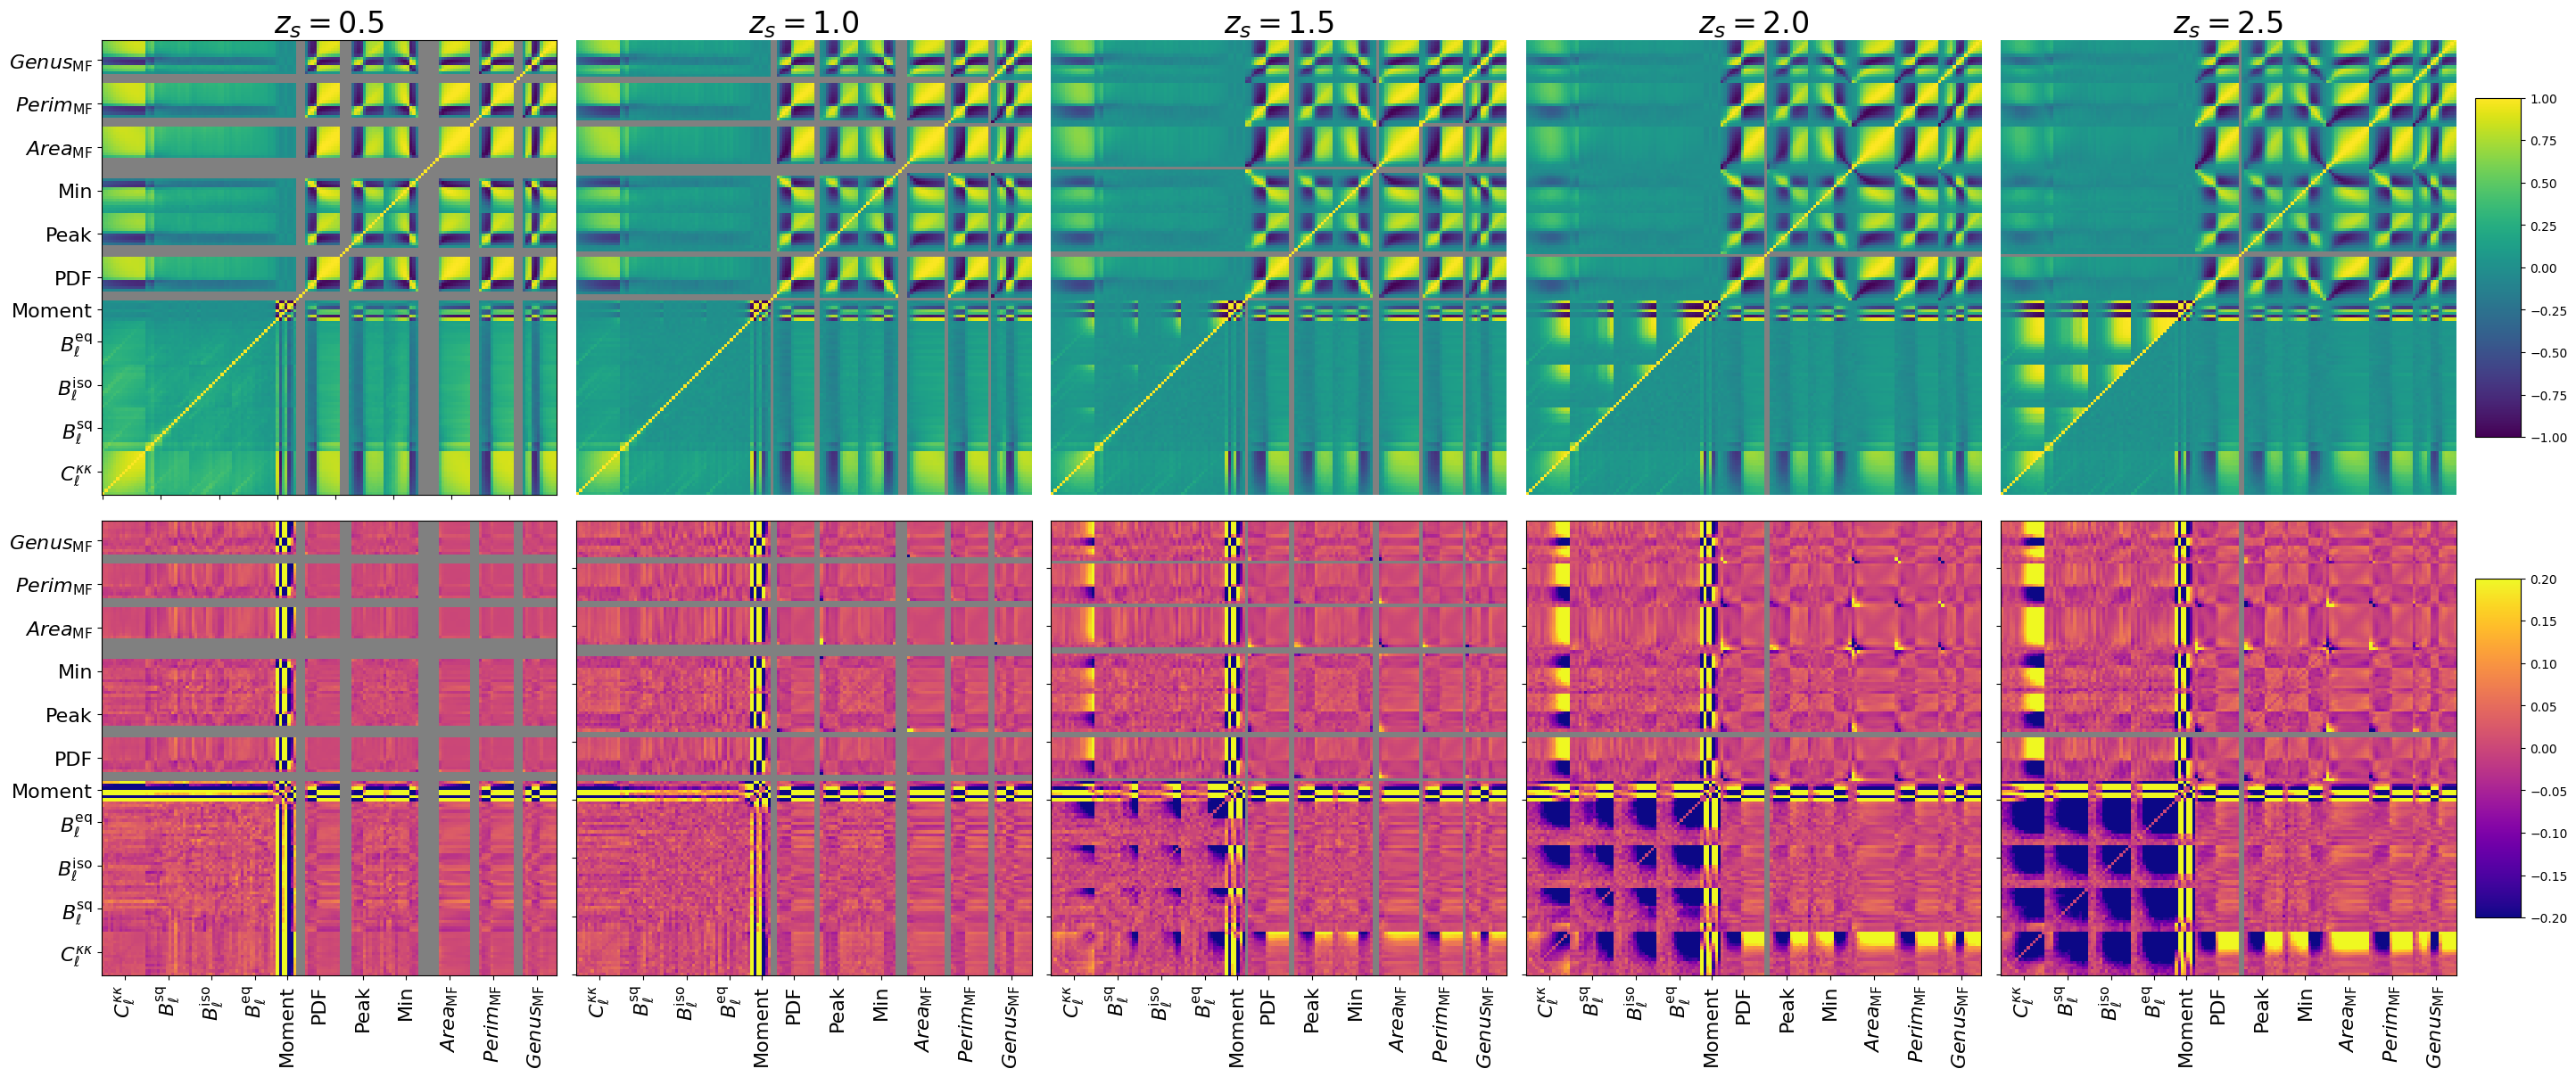
\includegraphics[width=\textwidth]{figures/corr_noiseless_final.png}
    \caption{Correlation matrices for various statistics at different source redshifts. In each panel of the top row, the left-upper triangle represents the TILED simulation, and the right-lower triangle represents the BIGBOX simulation. The bottom row shows the difference between the TILED and BIGBOX correlation matrices. Tiling effects are prominent in the high-$\ell$ regime of the power spectrum and bispectra, particularly in the off-diagonal elements, while non-correlation functions (PDF, peak counts, minima, and Minkowski Functionals) are less affected.}
    \label{fig:corr_noiseless}
\end{sidewaysfigure}

Conversely, Figure~\ref{fig:corr_ngal} illustrates the difference of noisy correlation matrix, incorporating the effects of galaxy shape noise. Each panel represents a different combination of source redshift and noise levels corresponding to current or upcoming surveys. The addition of noise diminishes the correlation structure in the high-$\ell$ regime of the power spectrum and bispectra, while the non-correlation functions remain comparatively unaffected.
\begin{figure}[h]
    \centering
    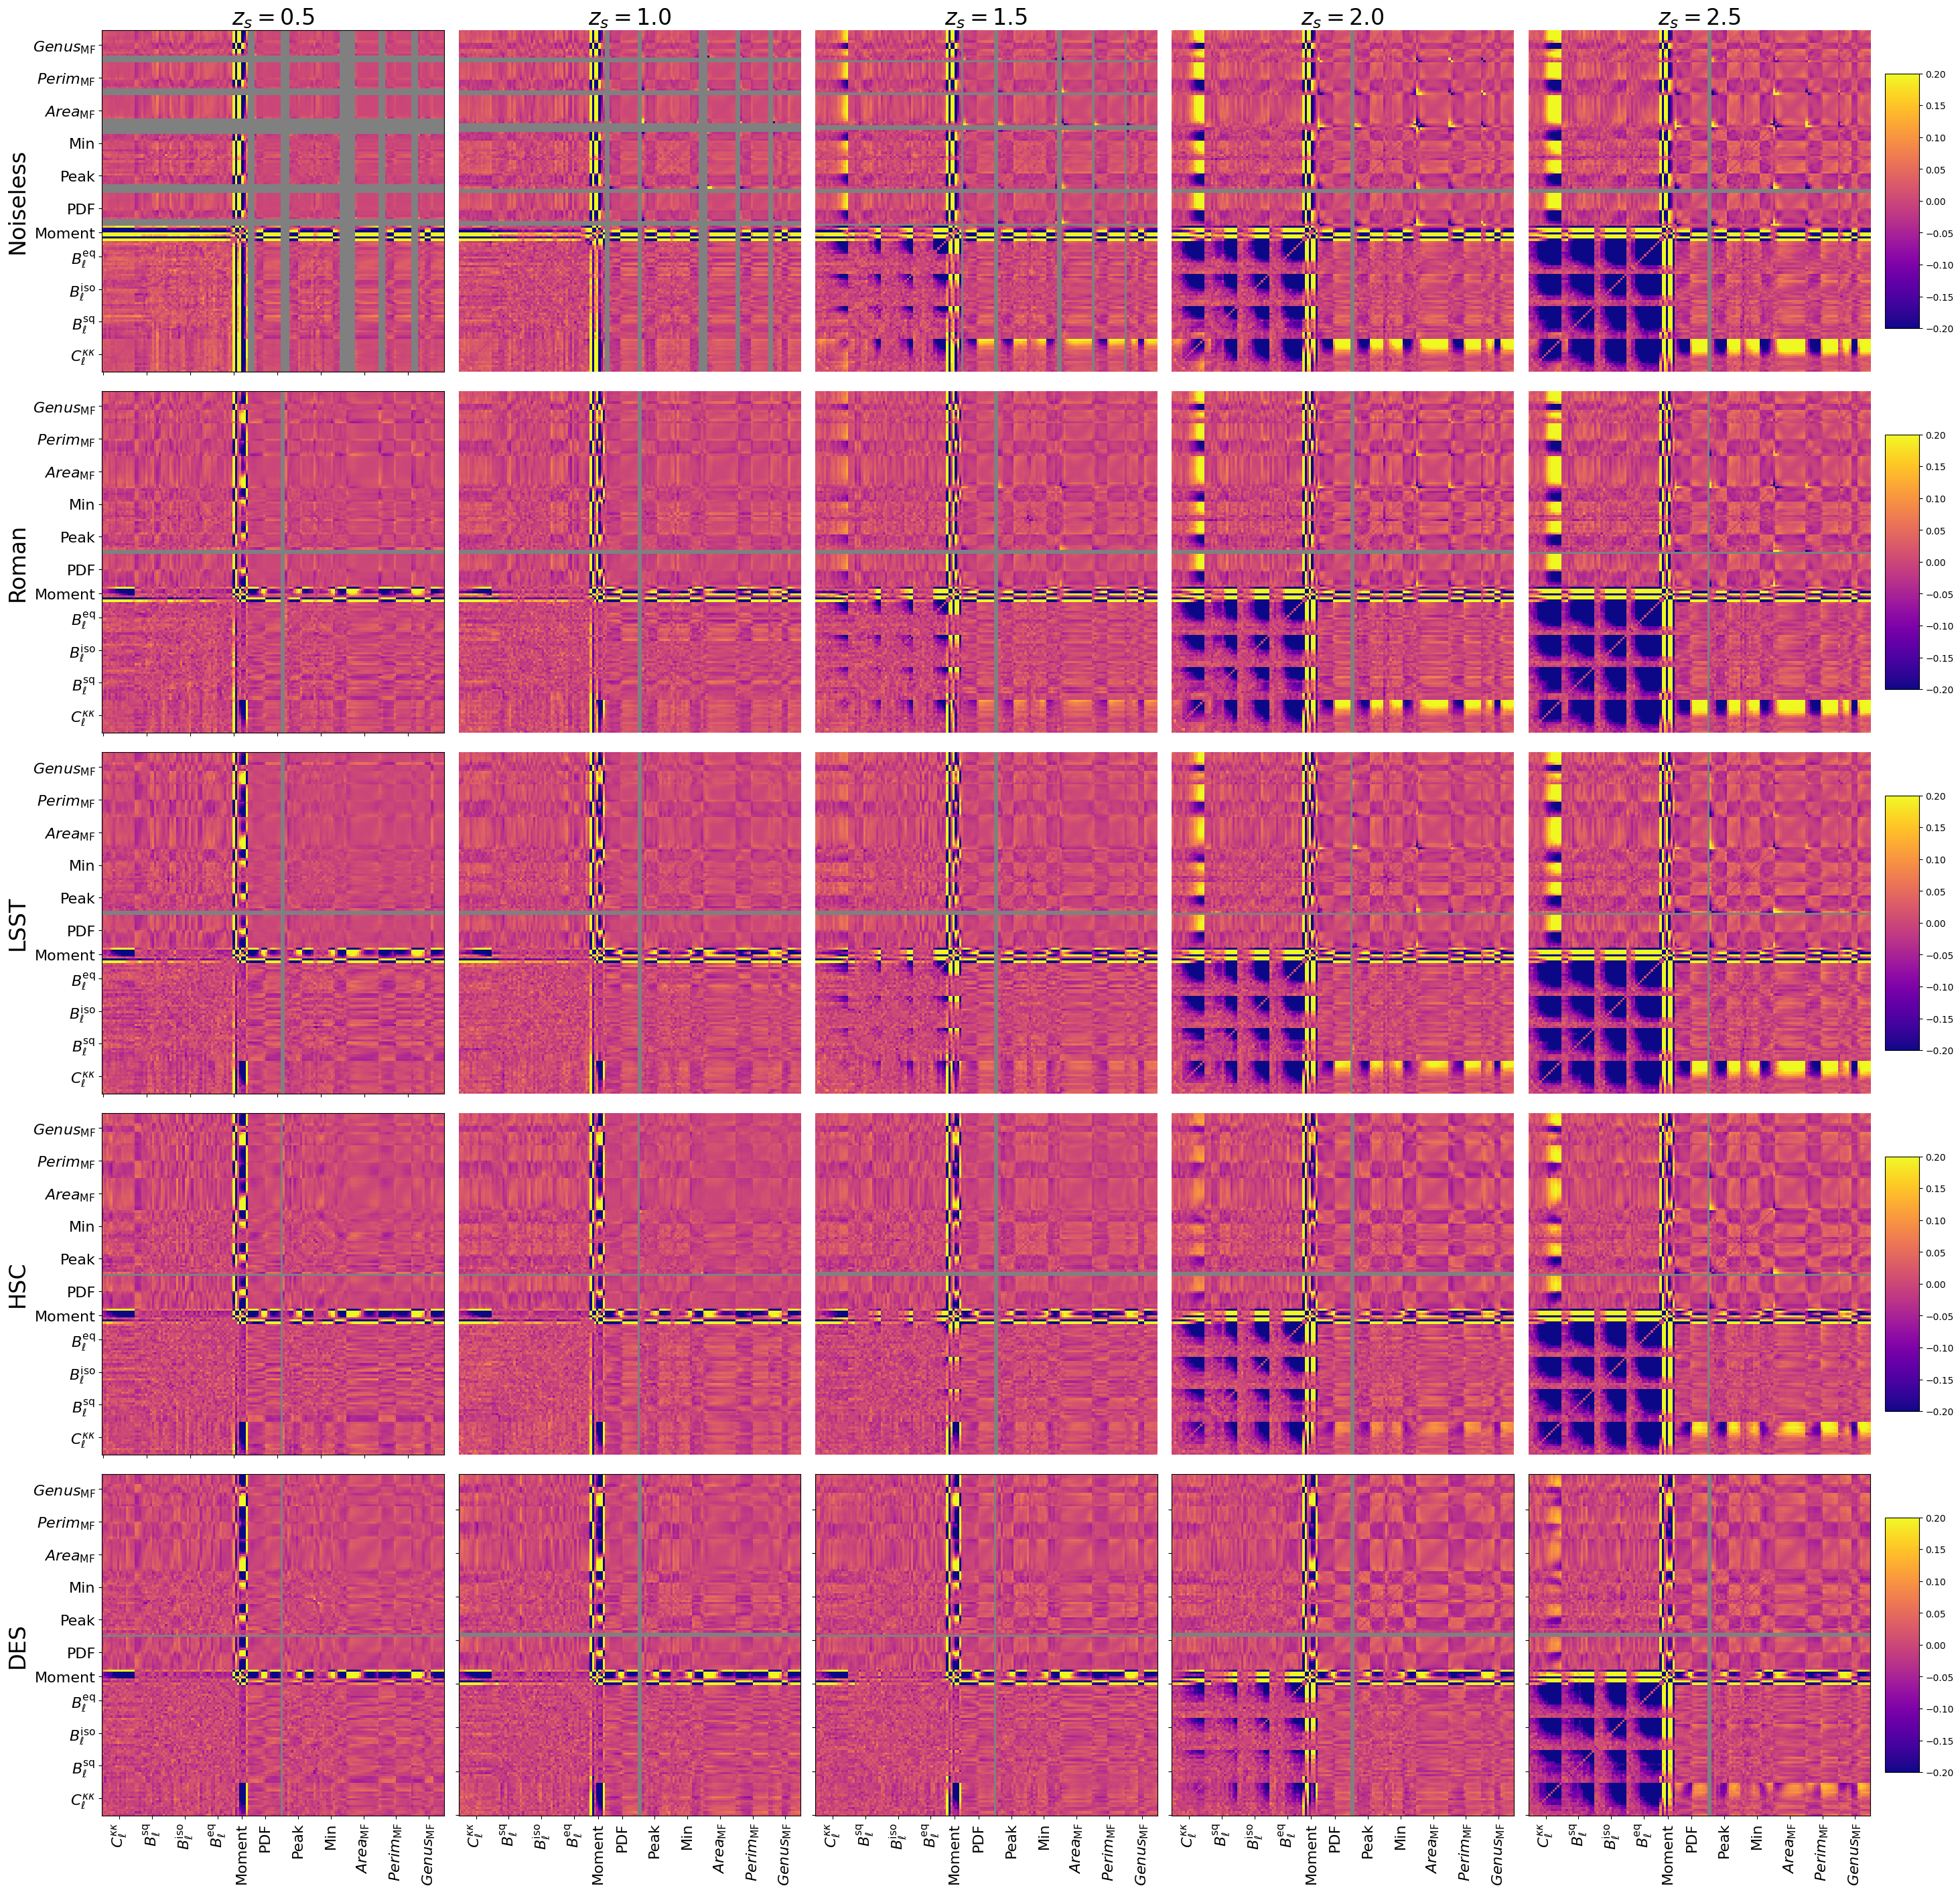
\includegraphics[width=\textwidth]{figures/corr_ngal_final.png}
    \caption{Noisy correlation matrices for various statistics at different source redshifts under different survey noise levels (Noiseless, Roman, LSST, HSC, DES). Galaxy shape noise diminishes the correlation structure in the high-$\ell$ regime of the power spectrum and bispectra, while non-correlation functions (PDF, peak counts, minima, and Minkowski Functionals) are less affected.}
    \label{fig:corr_ngal}
\end{figure}

\section{Comparison with theroretical models}
\subsection{Power Spectrum}
via halofit, 

\subsection{Bispectrum}
via bihalofit,

\subsection{PDF}
via hmpdf

\subsection{Peak Counts}
via gaussian prediction

\subsection{Minkowski Functionals}
via gaussian prediction